%\setchapterimage{bandeau}
\chapter*{Colle \arabic{cptColle} \\ 
Interface maître et esclave d'un robot -- 
\ifprof Corrigé \else Sujet \fi}
\addcontentsline{toc}{section}{Colle \arabic{cptColle} :
Interface maître et esclave d'un robot -- 
\ifprof Corrigé \else Sujet \fi}

\iflivret \stepcounter{cptColle} \else
\ifprof  \stepcounter{cptColle} \else \fi
\fi

\setcounter{question}{0}
\marginnote{CCP PSI 2015.}
%\marginnote[1cm]{
%\UPSTIcompetence[2]{C1-02}
%\UPSTIcompetence[2]{C2-04}}

%\begin{marginfigure}[4cm]
%\centering
%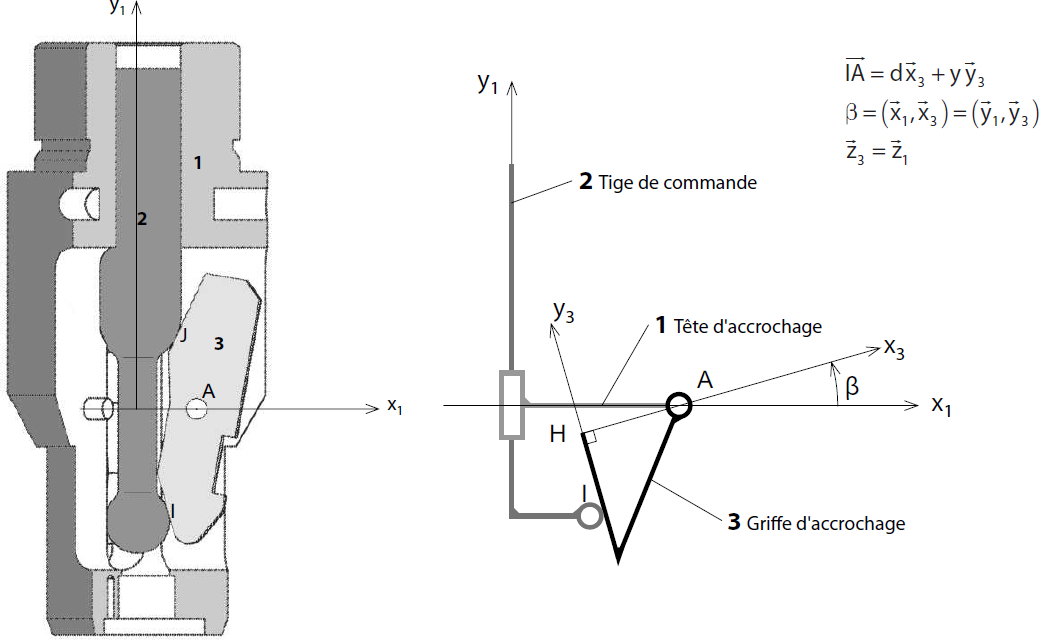
\includegraphics[width=4cm]{fig_01}
%\end{marginfigure}






\section*{Mise en situation}
\ifprof
\else
La téléopération consiste à mettre en relation deux manipulateurs appelés communément
maître et esclave. Le manipulateur maître permet au chirurgien de donner sa consigne de
déplacement à l’aide d’un levier de commande tandis que l’esclave l’exécute au contact de
l’environnement (l’organe à opérer). Les deux sous-systèmes échangent des informations de
déplacement et d’effort au travers d’un ou plusieurs canaux de communication. Un retour
visuel est également mis en place en parallèle à ce dispositif.

\begin{center}
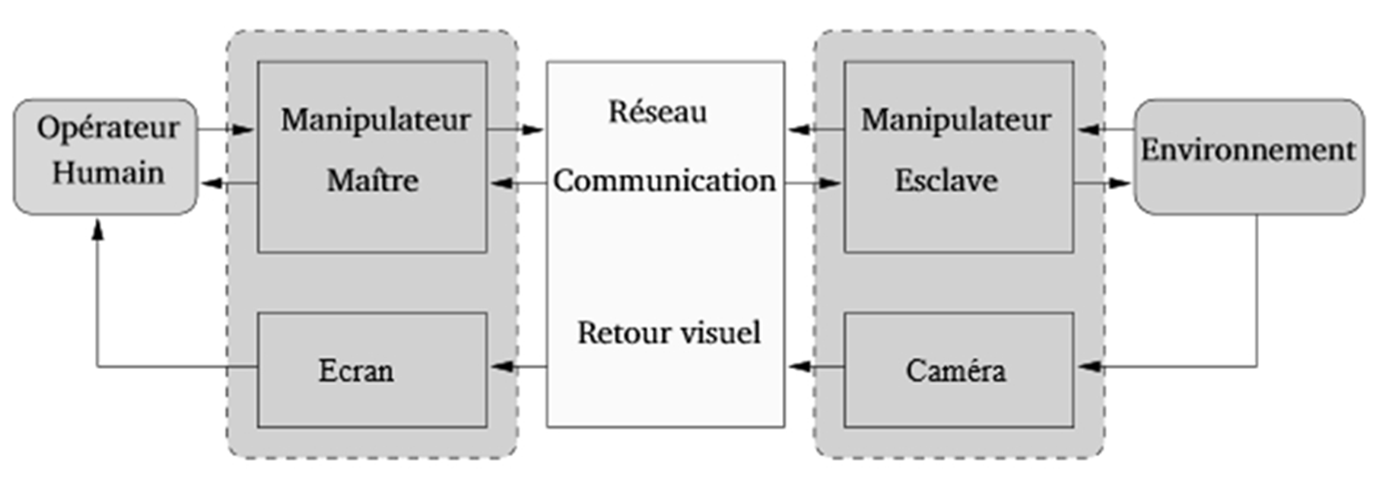
\includegraphics[width=\linewidth]{fig_00a}
%\textit{}
\end{center}
\fi
\begin{marginfigure}
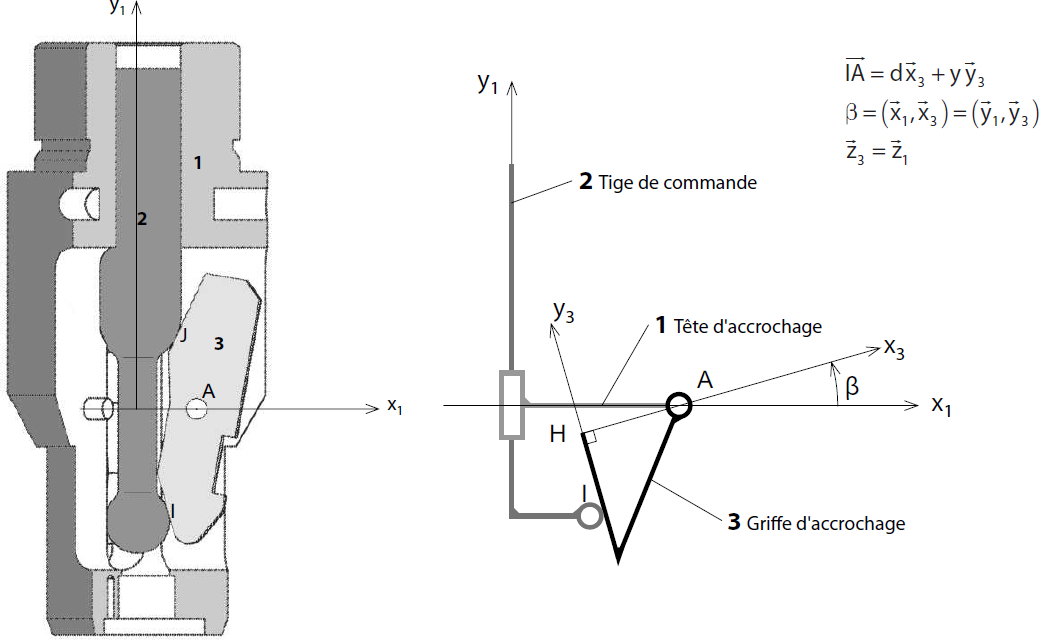
\includegraphics[width=\linewidth]{fig_01}
%\textit{}
\end{marginfigure}

\section*{Modélisation de l’interface maître}
\ifprof
\else

Ce mécanisme est constitué de 4 barres reliées par des liaisons pivots.



\begin{obj}
Vérifier que les exigences « Amplitude déplacement » (id 1.2.1.1), « Mouvement
rectiligne » (id 1.2.1.2), « Linéarité déplacement » (id 1.2.1.3) peuvent être satisfaites par le mécanisme de HOEKEN.
\end{obj}


\begin{center}
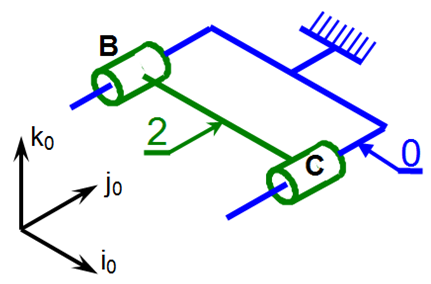
\includegraphics[width=.8\linewidth]{fig_02}
%\textit{}
\end{center}

\marginnote{
\begin{itemize}
\item Solide $S_0$, repère $\rep{0}\repere{A}{x_0}{y_0}{z_0}$, $\vect{AB}=L_0\vect{x_0}$ avec $L_0 = \SI{50}{mm}$.
\item Solide $S_1$, repère $\rep{1}\repere{B}{x_1}{y_1}{z_0}$, $\vect{BC}=L_1\vect{x_1}$ avec $L_1 = \SI{25}{mm}$, $\theta_1=\angl{x_0}{x_1}=\angl{y_0}{y_1}$.
\item Solide $S_2$, repère $\rep{2}\repere{A}{x_2}{y_2}{z_0}$, $\vect{AD}=L_2\vect{x_2}$ avec $L_2 = \SI{62,5}{mm}$, $\theta_2=\angl{x_0}{x_2}=\angl{y_0}{y_2}$.
\item Solide $S_3$, repère $\rep{3}\repere{C}{x_3}{y_3}{z_0}$, $\vect{ED}=\vect{DC}=L_2\vect{x_3}$ avec  $\theta_3=\angl{x_0}{x_3}=\angl{y_0}{y_3}$.
\end{itemize}}

\fi

%En développant une fermeture géométrique en projection dans la base du repère $\rep{0}$, d
\question{Donner
une relation algébrique reliant les paramètres $L_0$, $L_1$, $L_2$, $\theta_1$ et $\theta_3$.}
\ifprof
\begin{corrige}~\\
\begin{center}
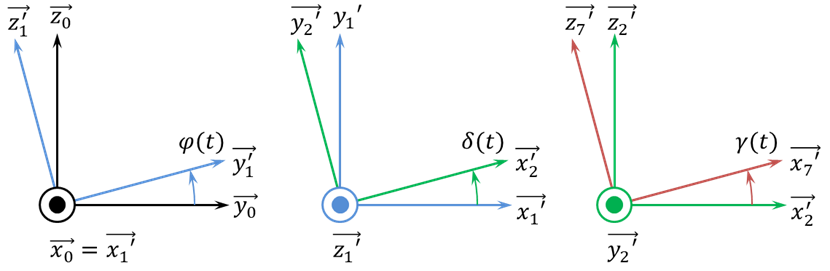
\includegraphics[width=\linewidth]{cor_01}
%\textit{}
\end{center}

En réalisant une fermeture géométrique on a $\vect{AB}+\vect{BC}+\vect{CD}+\vect{DA}=\vect{0}$.

On a alors, $L_0\vect{x_0}+L_1\vect{x_1}-L_2\vect{x_3}-L_2\vect{x_2}=\vect{0}$.

$\Leftrightarrow L_0\vect{x_0}+L_1\left( \cos \theta_1 \vect{x_0}+ \sin \theta_1 \vect{y_0} \right)-L_2\left( \cos \theta_3\vect{x_0} + \sin \theta_3\vect{y_0}  \right)-L_2\left( \cos \theta_2\vect{x_0} + \sin \theta_2\vect{y_0}  \right)=\vect{0}$.

En projetant dans la base $\mathcal{B}_0$, on a :

$
\left\{
\begin{array}{l}
L_0 + L_1 \cos \theta_1 -L_2\cos \theta_3-L_2 \cos \theta_2=0 \\
L_1\sin \theta_1-L_2 \sin \theta_3-L_2 \sin \theta_2=0 
\end{array} \right.
$

Il faut supprimer $\theta_2$ :

$
\left\{
\begin{array}{l}
L_0 + L_1 \cos \theta_1 -L_2\cos \theta_3=L_2 \cos \theta_2 \\
L_1\sin \theta_1-L_2 \sin \theta_3=L_2 \sin \theta_2
\end{array} \right.
$

En passant les expressions au carré et en les sommant, on a :

$\left(L_0 + L_1 \cos \theta_1 -L_2\cos \theta_3\right)^2 + \left( L_1\sin \theta_1-L_2 \sin \theta_3\right)^2=L_2^2 $


\end{corrige}
\else
\fi

\question{De même, exprimer le vecteur position du point $E$ ($\vect{AE}$) dans la base du repère $\rep{0}$ en fonction de $L_0$, $L_1$, $L_2$, $\theta_1$ et $\theta_3$.}
\ifprof
\begin{corrige}~\\
On a $\vect{AE}=\vect{AB}+\vect{BC}+\vect{CE}$ et donc 
 $\vect{AE}=L_0\vect{x_0}+L_1 \vect{x_1} -2L_2\vect{x_3}$. 
 
  $\vect{AE}=L_0\vect{x_0}+L_1\left( \cos \theta_1 \vect{x_0}+ \sin \theta_1 \vect{y_0} \right)-2L_2\left( \cos \theta_3\vect{x_0} + \sin \theta_3\vect{y_0}  \right)$. 
  
  Et $\vect{AE}=\begin{pmatrix} 
    L_0+L_1 \cos \theta_1 -2L_2\cos \theta_3 \\    
    L_1 \sin \theta_1 -2L_2 \sin \theta_3
  \end{pmatrix}_{\rep{0}}$
 
\end{corrige}
\else
\fi

\ifprof
\else

La résolution analytique du système d’équations permettant d’obtenir le déplacement du
point $E$ en fonction de l’angle de rotation $\theta_1$ du moteur et des différentes longueurs du mécanisme
n’étant pas triviale, seuls les résultats d’une simulation numérique seront analysés.

\begin{center}
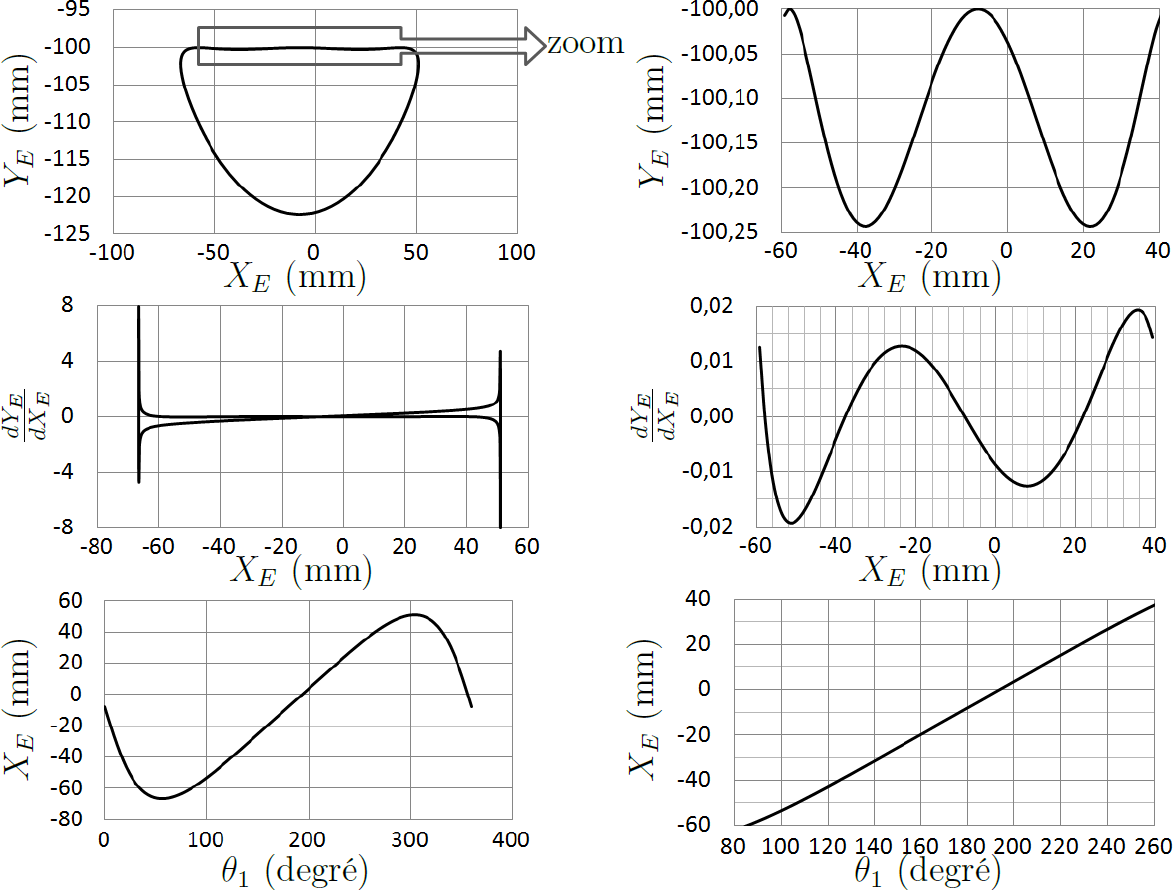
\includegraphics[width=\linewidth]{fig_03}
%\textit{}
\end{center}
\fi

\ifcolle
\else
\question{Vérifier, à l’aide des figures précédentes, que le déplacement du point $E$ est compatible avec les
exigences «~Amplitude déplacement~» (id 1.2.1.1) et «~Mouvement rectiligne~» (id 1.2.1.2) sur
l’intervalle $X_E \in \left[-\SI{60}{mm}; \SI{40}{mm}\right]$.}
\ifprof
\begin{corrige}~\\
\begin{itemize}
\item Amplitude déplacement de \SI{50}{mm} minimum : OK (amplitude de \SI{100}{mm}).
\item Mouvement rectiligne d'une amplitude $\Delta Y= \SI{0,5}{mm}$ maximum : OK (amplitude de \SI{0,25}{mm}).
\item Mouvement rectiligne d'une amplitude taux de variation $\dfrac{\dd Y_E}{\dd X_E}<\SI2\,\%$  : OK  (amplitude de $\pm 2\,\%$).
\end{itemize}
\end{corrige}
\else
\fi

\question{Proposer, à partir de la dernière figure, une démarche permettant de vérifier l’exigence « Linéarité
déplacement » (id 1.2.1.3) sur l’intervalle $X_E \in \left[-\SI{60}{mm}; \SI{40}{mm}\right]$.}
\ifprof
\begin{corrige}~\\
Il serait possible de faire une régression linéaire sur l'intervalle $\left[-\SI{60}{mm}; \SI{40}{mm}\right]$ et de vérifier que le coefficient de corrélation est supérieur à 0,99.
\end{corrige}
\else
\fi
\fi


\ifprof
\newpage
\else
\fi

\section*{Modélisation de l’interface esclave}
\ifprof
\else

\begin{marginfigure}
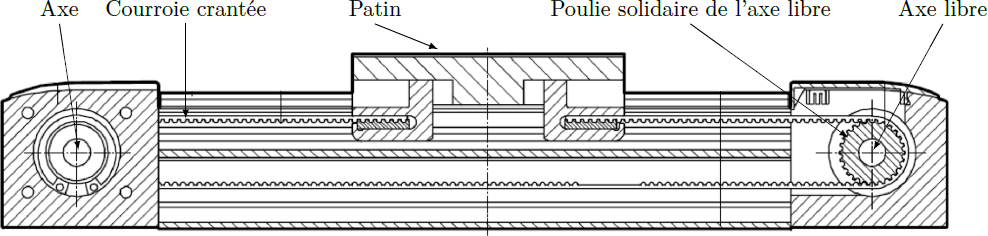
\includegraphics[width=\linewidth]{fig_04}
%\textit{}
\end{marginfigure}

\begin{marginfigure}
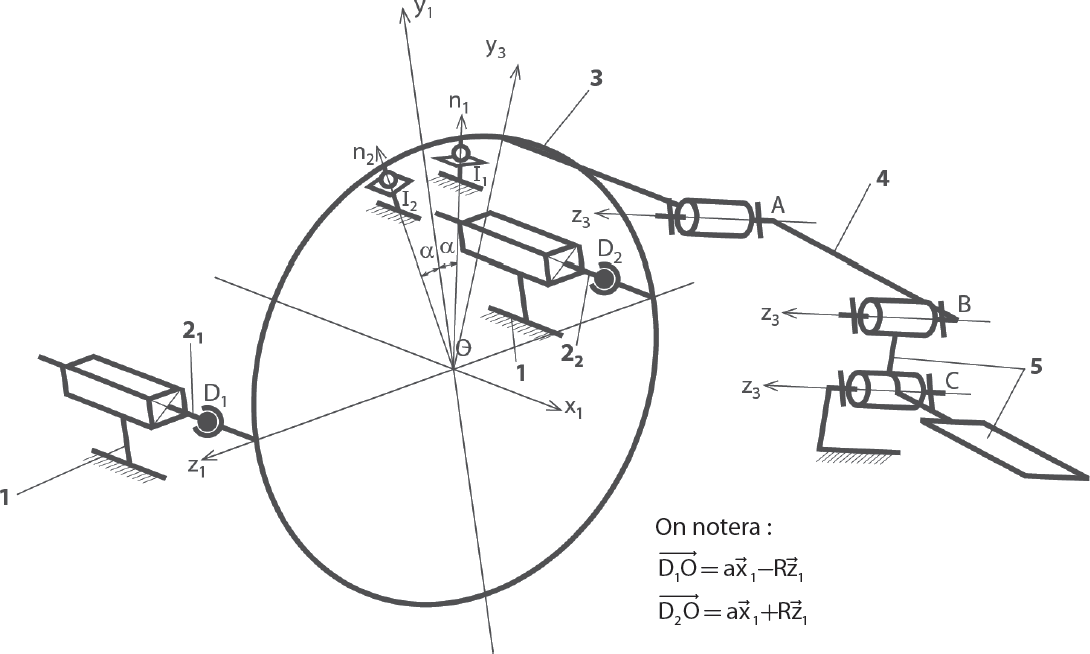
\includegraphics[width=\linewidth]{fig_05}
%\textit{}
\end{marginfigure}

\begin{center}
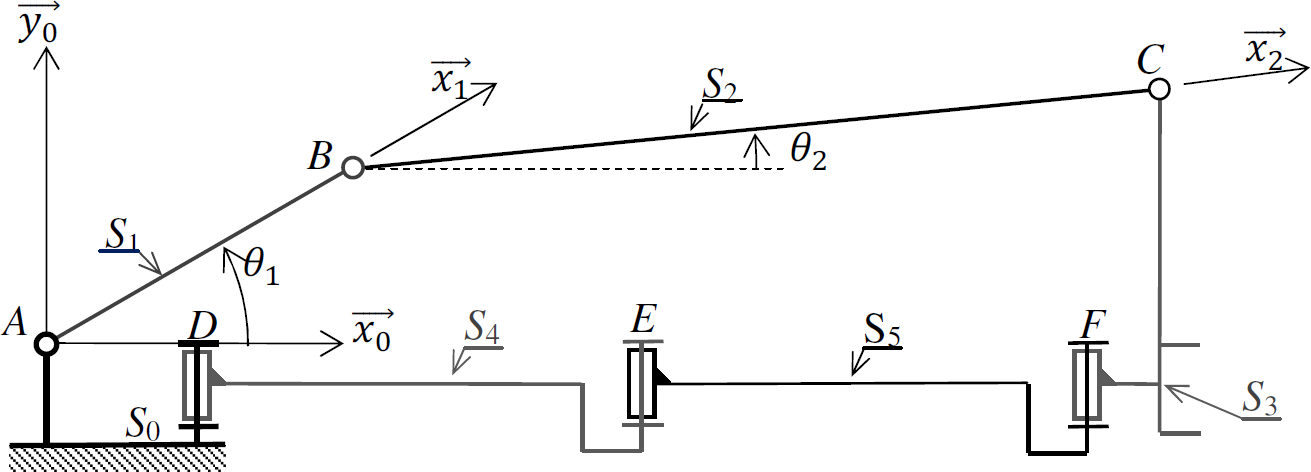
\includegraphics[width=.8\linewidth]{fig_06}
%\textit{}
\end{center}

\begin{center}
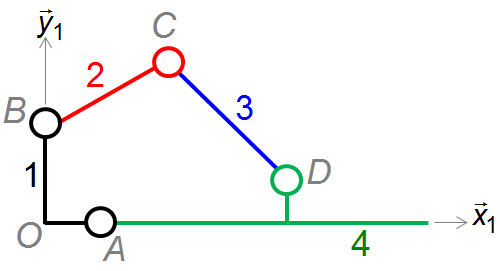
\includegraphics[width=\linewidth]{fig_07}
%\textit{}
\end{center}

\fi

\begin{obj}
Modéliser le comportement dynamique de l’interface esclave de façon à évaluer son
comportement au sein d’une boucle d’asservissement.
\end{obj}

\ifprof
\else

On note $\torseurstat{T}{\text{mot}}{S_1}=\torseurl{\vect{0}}{C_m\vect{z}}{\forall P}$ l’expression, dans la base $\mathcal{B}_0$ du torseur de l’action mécanique exercée par le moteur sur le solide $S_1$ et
l’accélération de la pesanteur sera représentée par le vecteur $\vect{g} = -g \vect{y_0}$.

\fi
\question{Tracer le graphe des liaisons du dispositif esclave. Précisier les actions mécaniques extéreiures Donner le degré d’hyperstatisme de la modélisation de ce mécanisme.}
\ifprof
\begin{corrige}~\\

\textbf{Méthode statique}
\begin{itemize}
\item Nombre de mobilité : $m=1$.
\item Nombre d'inconnues : 6 liaisons pivot. $I_S=30$. 
\item Nombre d'équations : 5 solides. $E_S = 30$. 
\item $h=m-E_S+I_S = 1-30+30=1$. 
\end{itemize}

\textbf{Méthode cinématique}

\begin{itemize}
\item Nombre de mobilité : $m=1$.
\item Nombre d'inconnues : 6 liaisons pivot. $I_c=6$. 
\item Nombre d'équations : 1 cycle. $E_c = 6$. 
\item $h=m-I_c+E_c = 1-6+6=1$. 
\end{itemize}

\end{corrige}
\else
\fi


\question{Proposer une modification simple pour le rendre isostatique.}
\ifprof
\begin{corrige}~\\
Pour rendre le système isostatique il faudrait ajouter une inconnue cinématique sans ajouter de mobilité. On peut par exemple remplacer une des liaison pivot par une liaison sphérique à doigt. 
\end{corrige}
\else
\fi


\question{Montrer que le mouvement de $S_3/S_0$ ne peut être qu’une translation de direction $\vect{x_0}$.}
\ifprof
\begin{corrige}~\\

D'une part, $\vecto{3}{0}=\vecto{3}{2}+\vecto{2}{1}+\vecto{1}{0}=\dot{\theta}_{30}\vect{z_0}$ (pivots parallèles d'axe $\vect{z_0}$).

D'autre part, $\vecto{3}{0}=\vecto{3}{5}+\vecto{5}{4}+\vecto{4}{0}=\dot{\theta}_{30}'\vect{y_0}$ (pivots parallèles d'axe $\vect{y_0}$).

On a donc $\dot{\theta}_{30}\vect{z_0} = \dot{\theta}_{30}'\vect{y_0}$ et donc nécessairement $\dot{\theta}_{30}=\dot{\theta}_{30}'=0$. 

Le mouvement de 3/0 est donc une translation. 
\end{corrige}
\else
\fi


\question{En utilisant le théorème de l’énergie cinétique, déterminer l’équation de mouvement liant
les paramètres $C_m$, $\dot{\theta}_1$, $\ddot{\theta}_1$, $\dot{x}_s$, $\ddot{x}_s$, $f_v$, $M_3$ et $I_1$.}
\ifprof
\begin{corrige}~\\
On isole $\Sigma = S_1 +S_2 + S_3 + S_4 + S_5$.

\textbf{Calcul de l'énergie cinétique :} $\ec{\Sigma}{0}=\ec{S_1}{0}+\ec{S_3}{0}$ car les masses et les inerties des autres solides sont négligés.  On a donc $\ec{\Sigma}{0}=\dfrac{1}{2}I_1\dot{\theta_1}^2 + \dfrac{1}{2}M_3 \vectv{C}{3}{0} ^2$ (car le mouvement de 3/0 est une translation. $\vectv{C}{3}{0}=\dfrac{\dd \vect{AC}}{\dd t}=\dot{x}_s \vect{x_0}$.

Au final, $\ec{\Sigma}{0}=\dfrac{1}{2}I_1\dot{\theta_1}^2 + \dfrac{1}{2}M_3\dot{x}_s ^2$.

\textbf{Bilan des puissances intérieures :} il n'y a pas de frottements; donc  $\mathcal{P}_{\text{int}}=0$.

\textbf{Bilan des puissances extérieures :}
\begin{itemize}
\item $\pext{\text{pes}}{3}=Mg\vect{y_0}\cdot \dot{x}_s \vect{x_0} = 0$;
\item $\pext{0}{1}{0}_{\text{mot}}=C_m\dot{\theta}_1$;
\item $\pext{0}{1}{0}_{\text{frot}}=-f_v\dot{\theta}_1^2$.
\end{itemize}

\textbf{Application du théorème de l'énergie cinétique :} on a $\dfrac{\dd \ec{\Sigma}{0} }{\dd t}=\mathcal{P}_{\text{int}} + \pext{\overline{\Sigma}}{\Sigma}{0}$, et donc 

$ I_1\dot{\theta_1}\ddot{\theta_1} + M_3\dot{x}_s\ddot{x}_s =C_m\dot{\theta}_1 -f_v\dot{\theta}_1^2$.


\end{corrige}
\else
\fi


\question{La relation géométrique liant les paramètres $x_s$ et $\theta_1$ n’étant pas triviale, on propose de la
linéariser autour du point de fonctionnement par l’expression $\theta_1(t)\simeq \alpha x_s(t)$ avec $\alpha=-\SI{30}{m^{-1}}$. En déduire l’équation différentielle liant les paramètres $C_m$, $\dot{x}_s$, $\ddot{x}_s$, $f_v$, $M_3$, $I_1$ et $\alpha$.}
\ifprof
\begin{corrige}~\\
On a directement $ I_1\alpha \dot{x}_s(t)\alpha \ddot{x}_s(t) + M_3\dot{x}_s\ddot{x}_s(t) =C_m\alpha \dot{x}_s(t) -f_v\alpha^2\dot{ x_s(t)}^2$
$\Leftrightarrow 
 I_1\alpha^2 \ddot{x}_s(t) + M_3\ddot{x}_s =C_m\alpha  -f_v\alpha^2 \dot{x}_s(t)$
\end{corrige}
\else
\fi


\question{Donner, dans les conditions d’Heaviside et sous forme canonique, la fonction de transfert
modélisant le comportement dynamique du manipulateur esclave : $H(p) = \dfrac{X_s(p)}{C_m(p)}$ sachant que
$X_s(p) = \mathcal{L}\left[x_s(t)\right]$ et $C_m(p) = \mathcal{L}\left[c_m(t)\right]$. Faire l’application numérique.}
\ifprof
\begin{corrige}~\\
En transformanr l'équation dans le domaine de Laplace, on a : $I_1\alpha^2 p^2X_s(p) + M_3p^2X_s(p) =C_m(p)\alpha  -f_v\alpha^2 pX_s(p)$
$\Leftrightarrow X_s(p) \left(I_1\alpha^2 p^2+ M_3p^2+f_v\alpha^2 p\right) =C_m(p)\alpha  $
$\Leftrightarrow H(p) = \dfrac{\alpha}{p\left(\left(I_1\alpha^2+ M_3\right)p+f_v\alpha^2 \right)} $.
$\Leftrightarrow H(p) = \dfrac{1/\left(f_v\alpha\right)}{p\left(\dfrac{I_1\alpha^2+ M_3}{f_v\alpha^2}p+1 \right)} $.

On a alors $K=-20,83$, $\tau = \dfrac{0,0513+ 0,1}{1,44}=\SI{0,105}{s}$.
\end{corrige}
\else
\fi

